A partire dai requisiti appena descritti, in questa fase si costruisce lo schema concettuale attraverso il modello Entità-Relazione (ER). Questo schema permette di rappresentare graficamente i dati e i loro legami in modo rigoroso, rimanendo del tutto indipendente dall'implementazione fisica.

Di seguito viene presentato il diagramma ER completo relativo alla struttura dei dati della facoltà (Figura \ref{fig:er_schema}). Si noti che tutti i vincoli che per limiti intrinseci del modello grafico non possono essere espressi, vengono trattati nella sezione \ref{sec:vincoli-di-integrita-e-di-dominio}.

\begin{figure}[h!]
    \centering
    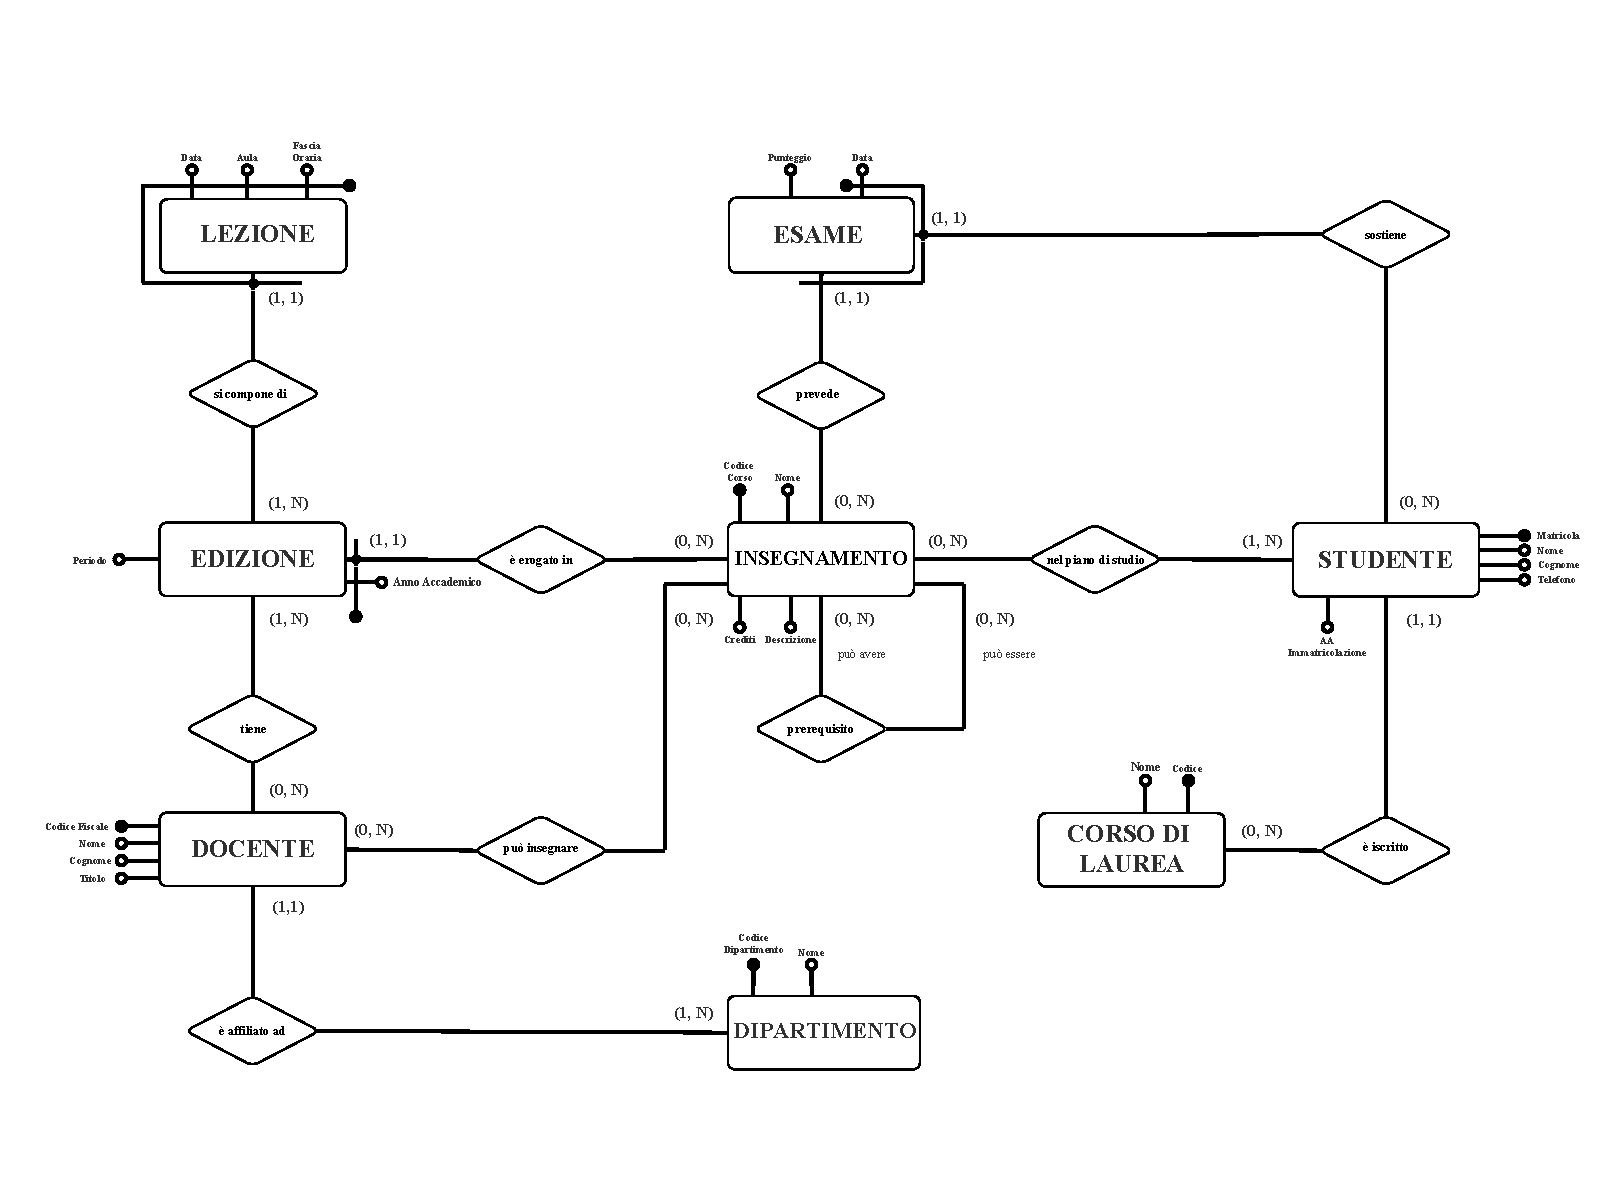
\includegraphics[width=\textwidth]{img/er.pdf}
    \caption{Schema ER per la gestione della didattica.}
    \label{fig:er_schema}
\end{figure}

\section{Vincoli di integrità e di dominio}
\label{sec:vincoli-di-integrita-e-di-dominio}

In questa sezione vengono descritte le regole che non si possono esprimere direttamente attraverso lo schema concettuale, ma che sono fondamentali per garantire che il sistema rispetti le regole della facoltà.

\subsection{Vincoli di propedeuticità}
\label{ssec:vincoli-di-propedeuticita}

\paragraph{Regola di precedenza degli esami}
Uno studente può registrare il superamento di una prova d'esame relativa a un insegnamento $I$ solo se risulta già certificato, per la medesima matricola, il superamento di tutti gli insegnamenti definiti come prerequisiti per $I$. In questo modo viene garantito il rispetto del corretto ordine di avanzamento della carriera.

\subsection{Vincoli temporali e di assegnazione}
\label{ssec:vincoli-temporali-e-di-assegnazione}

\paragraph{Unicità dell'edizione annuale}
Per ogni insegnamento presente nell'offerta formativa, non può essere attivata più di un'edizione nel medesimo anno accademico.
Questo garantisce che la pianificazione didattica sia univoca su base annuale.

\paragraph{Vincolo di abilitazione alla docenza}
Un docente può assumere la titolarità di un'edizione solo se risulta formalmente abilitato a tenere quello specifico insegnamento.
Tale regola impedisce l'assegnazione di incarichi didattici al di fuori delle competenze certificate dalla facoltà.

\subsection{Specifiche sui domini dei dati}
\label{ssec:specifiche-sui-domini-dei-dati}

\paragraph{Restrizioni sui periodi didattici}
L'organizzazione temporale della didattica su scala annuale è soggetta a parametri rigidi imposti dalla facoltà. Nello specifico, il periodo didattico in cui si svolge un'edizione deve necessariamente appartenere all'insieme finito $\{1, 2, 3\}$.

\paragraph{Restrizioni sulle fasce orarie}
La collocazione giornaliera delle singole lezioni segue vincoli logistici altrettanto restrittivi.
Tale parametro è infatti strettamente limitato a quattro blocchi temporali predefiniti, identificati dai valori discreti $\{1, 2, 3, 4\}$.

\paragraph{Restrizioni sui giorni di lezione}
Per garantire la coerenza del calendario didattico, la programmazione settimanale esclude i fine settimana.
Di conseguenza, il valore relativo al giorno in cui si svolge una lezione è rigorosamente limitato all'insieme testuale \{Lunedì, Martedì, Mercoledì, Giovedì, Venerdì\}.

\paragraph{Restrizioni sul titolo accademico}
Mentre il dipartimento di afferenza è gestito tramite un'entità dedicata, il titolo del docente è modellato come un dominio vincolato. Questa scelta dipende dalla natura statica del dato, che cambia molto raramente nel tempo. Il titolo deve quindi appartenere a un elenco chiuso di valori, come $\{Ricercatore, Professore Associato, Professore Ordinario\}$.
